%!TEX TS-program = xelatex
% NOTE: as of 17 Sept 2012, this compiles in xelatex

\documentclass{beamer}
\usepackage{etoolbox}
\makeatletter
\patchcmd{\slideentry}{\ifnum#2>0}{\ifnum2>0}{}{\@error{unable to patch}}
\makeatother

\usetheme{Frankfurt}
\setbeamercovered{invisible}
\setbeamertemplate{navigation symbols}{} 

\usepackage{coordsys} % for number lines
\usepackage{graphicx}
\usepackage{multirow}
\usepackage{caption}
\usepackage{subfig}
\usepackage{tikz}

%%%%%%%%%%%%%%%%%%%%%%%%%%%%%%%%%%%%%%%%%
\title[Regime Classification \hspace{14em} \insertframenumber/
\inserttotalframenumber]{Probabilistic Measures of \\ Regime Type}
\author{Shahryar Minhas}
\institute[Duke University]
{
{\emph{sfm12@duke.edu}} \\
\medskip
Duke University 
}
\date{\today}

\begin{document}

%%%%%%%%%%%%%%%%%%%%%%%%%%%%%%%%%%%%%%%%%
\begin{frame}
\titlepage
\end{frame}
%%%%%%%%%%%%%%%%%%%%%%%%%%%%%%%%%%%%%%%%%

\section{Overview}

%%%%%%%%%%%%%%%%%%%%%%%%%%%%%%%%%%%%%%%%%
\begin{frame}
\frametitle{Goal}

Create country/year probabilistic measures of archetypical regime types, specifically:

\begin{itemize}
	\item Democracy
	\item Militaristic	
	\item Monarchical
	\item One-Party
\end{itemize}

\end{frame}
%%%%%%%%%%%%%%%%%%%%%%%%%%%%%%%%%%%%%%%%%

%%%%%%%%%%%%%%%%%%%%%%%%%%%%%%%%%%%%%%%%%
\begin{frame}
\frametitle{Method: Supervised Approaches}

\begin{itemize}
	\item Bernoulli Naive Bayes
	\item Support Vector Machines (SVM)
\end{itemize}

\end{frame}
%%%%%%%%%%%%%%%%%%%%%%%%%%%%%%%%%%%%%%%%%

\section{Data}

%%%%%%%%%%%%%%%%%%%%%%%%%%%%%%%%%%%%%%%%%
\begin{frame}
\frametitle{Textual Data}

\begin{itemize}
	\item Scraped all country level reports for 1999-2013 from: 
		\begin{itemize}
			\item State Department Human Right Reports
			\item Freedom House Freedom in the World Reports
		\end{itemize}
	\item Cleaning textual data:
		\begin{itemize}
			\item Removed numbers, punctuation, and stopwords
			\item Tokenized results
			\item Lemmatized tokens to group together inflected forms
		\end{itemize}
\end{itemize}

\end{frame}
%%%%%%%%%%%%%%%%%%%%%%%%%%%%%%%%%%%%%%%%%

%%%%%%%%%%%%%%%%%%%%%%%%%%%%%%%%%%%%%%%%%
\begin{frame}
\frametitle{Datasets used for Labels}

\begin{itemize}
	\item Marshall et al. 2014 (Polity)
	\item Freedom House 2014 (FH)
	\item Geddes et al. 2014 (GWF)
	\item Hadenius et al. 2012 (ADR)
\end{itemize}

\end{frame}
%%%%%%%%%%%%%%%%%%%%%%%%%%%%%%%%%%%%%%%%%

%%%%%%%%%%%%%%%%%%%%%%%%%%%%%%%%%%%%%%%%%
\begin{frame}
\frametitle{Label Rules}

\begin{block}{Democracy}
If Polity equals 10 and FH equals Free then we set Democracy for country-year equal to one otherwise zero
\end{block}

\begin{block}{Military, Monarchy, \& Party}
If GWF and ADR dataset agree on coding for country-year then variable equals one otherwise zero
\end{block}

\end{frame}
%%%%%%%%%%%%%%%%%%%%%%%%%%%%%%%%%%%%%%%%%

\section{Empirics}

%%%%%%%%%%%%%%%%%%%%%%%%%%%%%%%%%%%%%%%%%
\begin{frame}
\frametitle{Cross-Validation Strategy}

\begin{block}{Democracy}
\begin{itemize}
	\item Training dataset: 1,557 cases from 1999-2008 
	\item Test dataset: 707 cases from 2009-2013
\end{itemize}
\end{block}

\begin{block}{Military, Monarchy, \& Party}
\begin{itemize}
	\item Training dataset: 1,138 cases from 1999-2006 
	\item Test dataset: 583 cases from 2007-2010
	\item Shorter timeline because GWF and ADR datasets end at 2010
\end{itemize}
\end{block}

\end{frame}
%%%%%%%%%%%%%%%%%%%%%%%%%%%%%%%%%%%%%%%%%

%%%%%%%%%%%%%%%%%%%%%%%%%%%%%%%%%%%%%%%%%
\begin{frame}
\frametitle{Label Distributions}

\begin{figure}[ht]
	\centering
	\resizebox{1\textwidth}{!}{% Created by tikzDevice version 0.7.0 on 2014-08-06 05:29:37
% !TEX encoding = UTF-8 Unicode
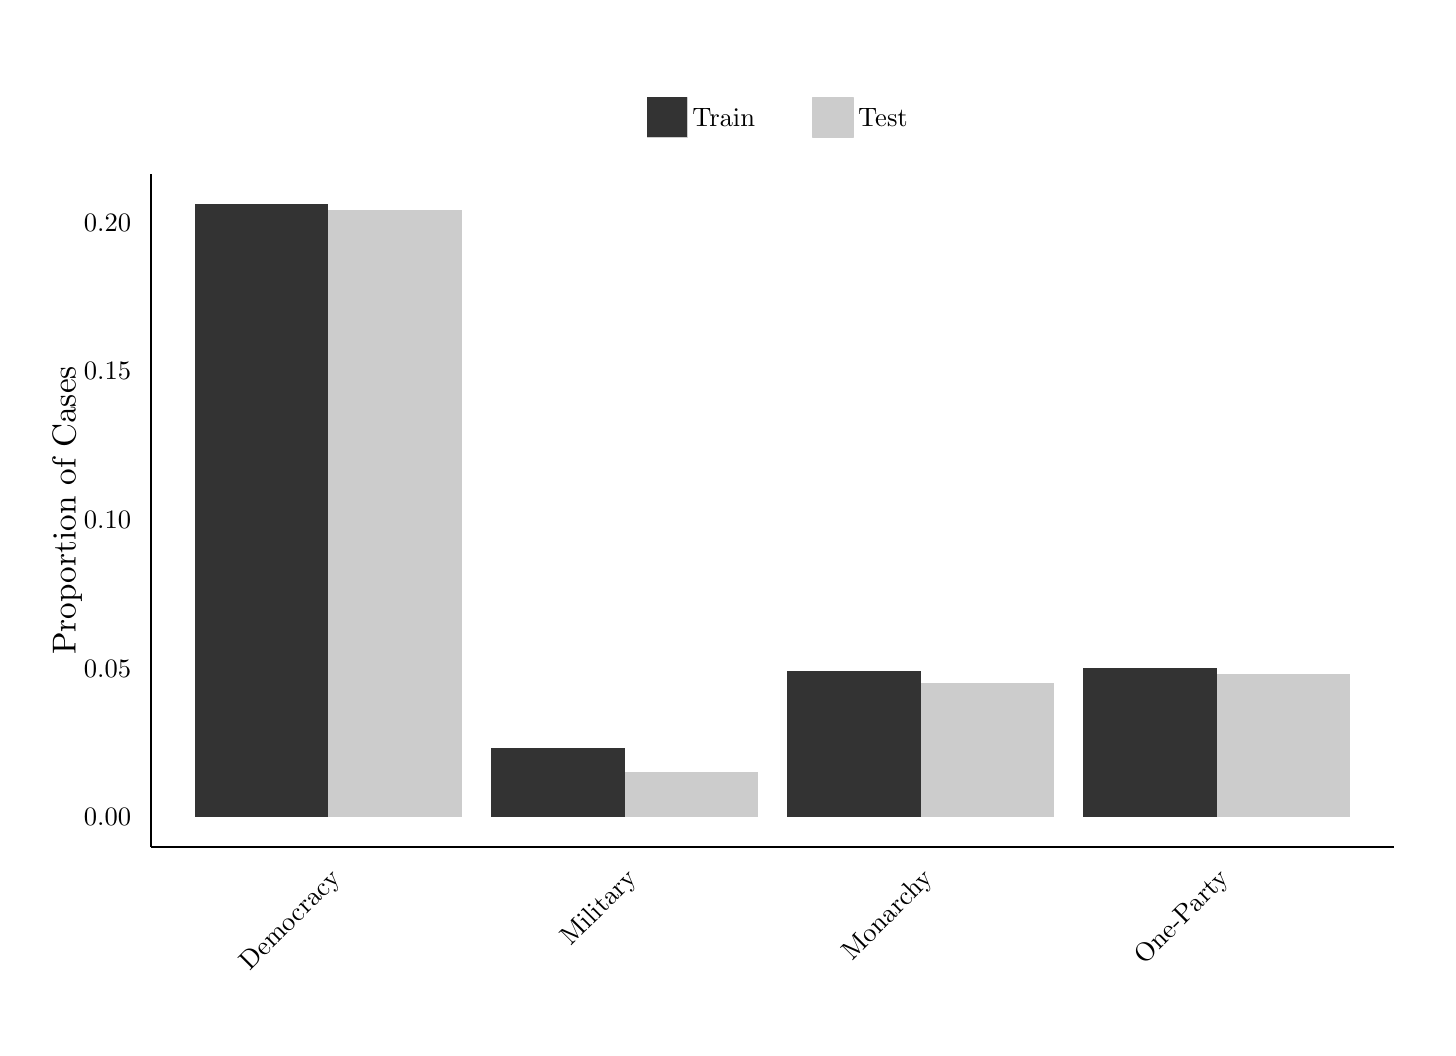
\begin{tikzpicture}[x=1pt,y=1pt]
\definecolor[named]{fillColor}{rgb}{1.00,1.00,1.00}
\path[use as bounding box,fill=fillColor,fill opacity=0.00] (0,0) rectangle (505.89,361.35);
\begin{scope}
\path[clip] (  0.00,  0.00) rectangle (505.89,361.35);
\definecolor[named]{drawColor}{rgb}{1.00,1.00,1.00}
\definecolor[named]{fillColor}{rgb}{1.00,1.00,1.00}

\path[draw=drawColor,line width= 0.6pt,line join=round,line cap=round,fill=fillColor] (  0.00,  0.00) rectangle (505.89,361.35);
\end{scope}
\begin{scope}
\path[clip] ( 44.49, 65.20) rectangle (493.85,308.58);
\definecolor[named]{fillColor}{rgb}{1.00,1.00,1.00}

\path[fill=fillColor] ( 44.49, 65.20) rectangle (493.85,308.58);
\definecolor[named]{fillColor}{rgb}{0.20,0.20,0.20}

\path[fill=fillColor] ( 60.53, 76.26) rectangle (108.68,297.52);
\definecolor[named]{fillColor}{rgb}{0.80,0.80,0.80}

\path[fill=fillColor] (108.68, 76.26) rectangle (156.83,295.37);
\definecolor[named]{fillColor}{rgb}{0.20,0.20,0.20}

\path[fill=fillColor] (167.52, 76.26) rectangle (215.67,100.97);
\definecolor[named]{fillColor}{rgb}{0.80,0.80,0.80}

\path[fill=fillColor] (215.67, 76.26) rectangle (263.82, 92.37);
\definecolor[named]{fillColor}{rgb}{0.20,0.20,0.20}

\path[fill=fillColor] (274.51, 76.26) rectangle (322.66,128.89);
\definecolor[named]{fillColor}{rgb}{0.80,0.80,0.80}

\path[fill=fillColor] (322.66, 76.26) rectangle (370.81,124.60);
\definecolor[named]{fillColor}{rgb}{0.20,0.20,0.20}

\path[fill=fillColor] (381.51, 76.26) rectangle (429.65,129.97);
\definecolor[named]{fillColor}{rgb}{0.80,0.80,0.80}

\path[fill=fillColor] (429.65, 76.26) rectangle (477.80,127.82);
\end{scope}
\begin{scope}
\path[clip] (  0.00,  0.00) rectangle (505.89,361.35);
\definecolor[named]{drawColor}{rgb}{0.00,0.00,0.00}

\path[draw=drawColor,line width= 0.6pt,line join=round] ( 44.49, 65.20) --
	( 44.49,308.58);
\end{scope}
\begin{scope}
\path[clip] (  0.00,  0.00) rectangle (505.89,361.35);
\definecolor[named]{drawColor}{rgb}{0.00,0.00,0.00}

\node[text=drawColor,anchor=base east,inner sep=0pt, outer sep=0pt, scale=  0.96] at ( 37.37, 72.96) {0.00};

\node[text=drawColor,anchor=base east,inner sep=0pt, outer sep=0pt, scale=  0.96] at ( 37.37,126.66) {0.05};

\node[text=drawColor,anchor=base east,inner sep=0pt, outer sep=0pt, scale=  0.96] at ( 37.37,180.36) {0.10};

\node[text=drawColor,anchor=base east,inner sep=0pt, outer sep=0pt, scale=  0.96] at ( 37.37,234.06) {0.15};

\node[text=drawColor,anchor=base east,inner sep=0pt, outer sep=0pt, scale=  0.96] at ( 37.37,287.77) {0.20};
\end{scope}
\begin{scope}
\path[clip] (  0.00,  0.00) rectangle (505.89,361.35);
\definecolor[named]{drawColor}{rgb}{0.00,0.00,0.00}

\path[draw=drawColor,line width= 0.6pt,line join=round] ( 44.49, 65.20) --
	(493.85, 65.20);
\end{scope}
\begin{scope}
\path[clip] (  0.00,  0.00) rectangle (505.89,361.35);
\definecolor[named]{drawColor}{rgb}{0.00,0.00,0.00}

\node[text=drawColor,rotate= 45.00,anchor=base east,inner sep=0pt, outer sep=0pt, scale=  0.96] at (113.35, 53.41) {Democracy};

\node[text=drawColor,rotate= 45.00,anchor=base east,inner sep=0pt, outer sep=0pt, scale=  0.96] at (220.35, 53.41) {Military};

\node[text=drawColor,rotate= 45.00,anchor=base east,inner sep=0pt, outer sep=0pt, scale=  0.96] at (327.34, 53.41) {Monarchy};

\node[text=drawColor,rotate= 45.00,anchor=base east,inner sep=0pt, outer sep=0pt, scale=  0.96] at (434.33, 53.41) {One-Party};
\end{scope}
\begin{scope}
\path[clip] (  0.00,  0.00) rectangle (505.89,361.35);
\definecolor[named]{drawColor}{rgb}{0.00,0.00,0.00}

\node[text=drawColor,rotate= 90.00,anchor=base,inner sep=0pt, outer sep=0pt, scale=  1.20] at ( 17.30,186.89) {Proportion of Cases};
\end{scope}
\begin{scope}
\path[clip] (  0.00,  0.00) rectangle (505.89,361.35);
\definecolor[named]{fillColor}{rgb}{1.00,1.00,1.00}

\path[fill=fillColor] (216.03,317.45) rectangle (322.30,340.44);
\end{scope}
\begin{scope}
\path[clip] (  0.00,  0.00) rectangle (505.89,361.35);
\definecolor[named]{drawColor}{rgb}{0.80,0.80,0.80}
\definecolor[named]{fillColor}{rgb}{1.00,1.00,1.00}

\path[draw=drawColor,line width= 0.6pt,line join=round,line cap=round,fill=fillColor] (223.91,321.72) rectangle (238.36,336.17);
\end{scope}
\begin{scope}
\path[clip] (  0.00,  0.00) rectangle (505.89,361.35);
\definecolor[named]{fillColor}{rgb}{0.20,0.20,0.20}

\path[fill=fillColor] (223.91,321.72) rectangle (238.36,336.17);

\path[] (223.91,321.72) --
	(238.36,336.17);
\end{scope}
\begin{scope}
\path[clip] (  0.00,  0.00) rectangle (505.89,361.35);
\definecolor[named]{drawColor}{rgb}{0.80,0.80,0.80}
\definecolor[named]{fillColor}{rgb}{1.00,1.00,1.00}

\path[draw=drawColor,line width= 0.6pt,line join=round,line cap=round,fill=fillColor] (283.86,321.72) rectangle (298.31,336.17);
\end{scope}
\begin{scope}
\path[clip] (  0.00,  0.00) rectangle (505.89,361.35);
\definecolor[named]{fillColor}{rgb}{0.80,0.80,0.80}

\path[fill=fillColor] (283.86,321.72) rectangle (298.31,336.17);

\path[] (283.86,321.72) --
	(298.31,336.17);
\end{scope}
\begin{scope}
\path[clip] (  0.00,  0.00) rectangle (505.89,361.35);
\definecolor[named]{drawColor}{rgb}{0.00,0.00,0.00}

\node[text=drawColor,anchor=base west,inner sep=0pt, outer sep=0pt, scale=  0.96] at (240.17,325.64) {Train\qquad\qquad};
\end{scope}
\begin{scope}
\path[clip] (  0.00,  0.00) rectangle (505.89,361.35);
\definecolor[named]{drawColor}{rgb}{0.00,0.00,0.00}

\node[text=drawColor,anchor=base west,inner sep=0pt, outer sep=0pt, scale=  0.96] at (300.12,325.64) {Test};
\end{scope}
\end{tikzpicture}
}	
\end{figure}

\end{frame}
%%%%%%%%%%%%%%%%%%%%%%%%%%%%%%%%%%%%%%%%%

%%%%%%%%%%%%%%%%%%%%%%%%%%%%%%%%%%%%%%%%%
\begin{frame}
\frametitle{Features for Supervised Models}

\begin{itemize}
	\item Vectorized tokens from combined State and FH reports for a given country-year
	\item Experimented with additional features but supervised models with just vectorized tokens performed the best (in terms of precision, recall and accuracy), see below for other features attempted:
	\begin{itemize}
		\item Word count of combined tokens
		\item Posterior topic predictions from an unsupervised LDA
	\end{itemize}
\end{itemize}

\end{frame}
%%%%%%%%%%%%%%%%%%%%%%%%%%%%%%%%%%%%%%%%%

\section{Results}

%%%%%%%%%%%%%%%%%%%%%%%%%%%%%%%%%%%%%%%%%
\begin{frame}
\frametitle{Out-of-Sample Performance}

\begin{figure}[ht]
	\centering
	\resizebox{1\textwidth}{!}{% Created by tikzDevice version 0.6.2 on 2014-10-03 01:20:09
% !TEX encoding = UTF-8 Unicode
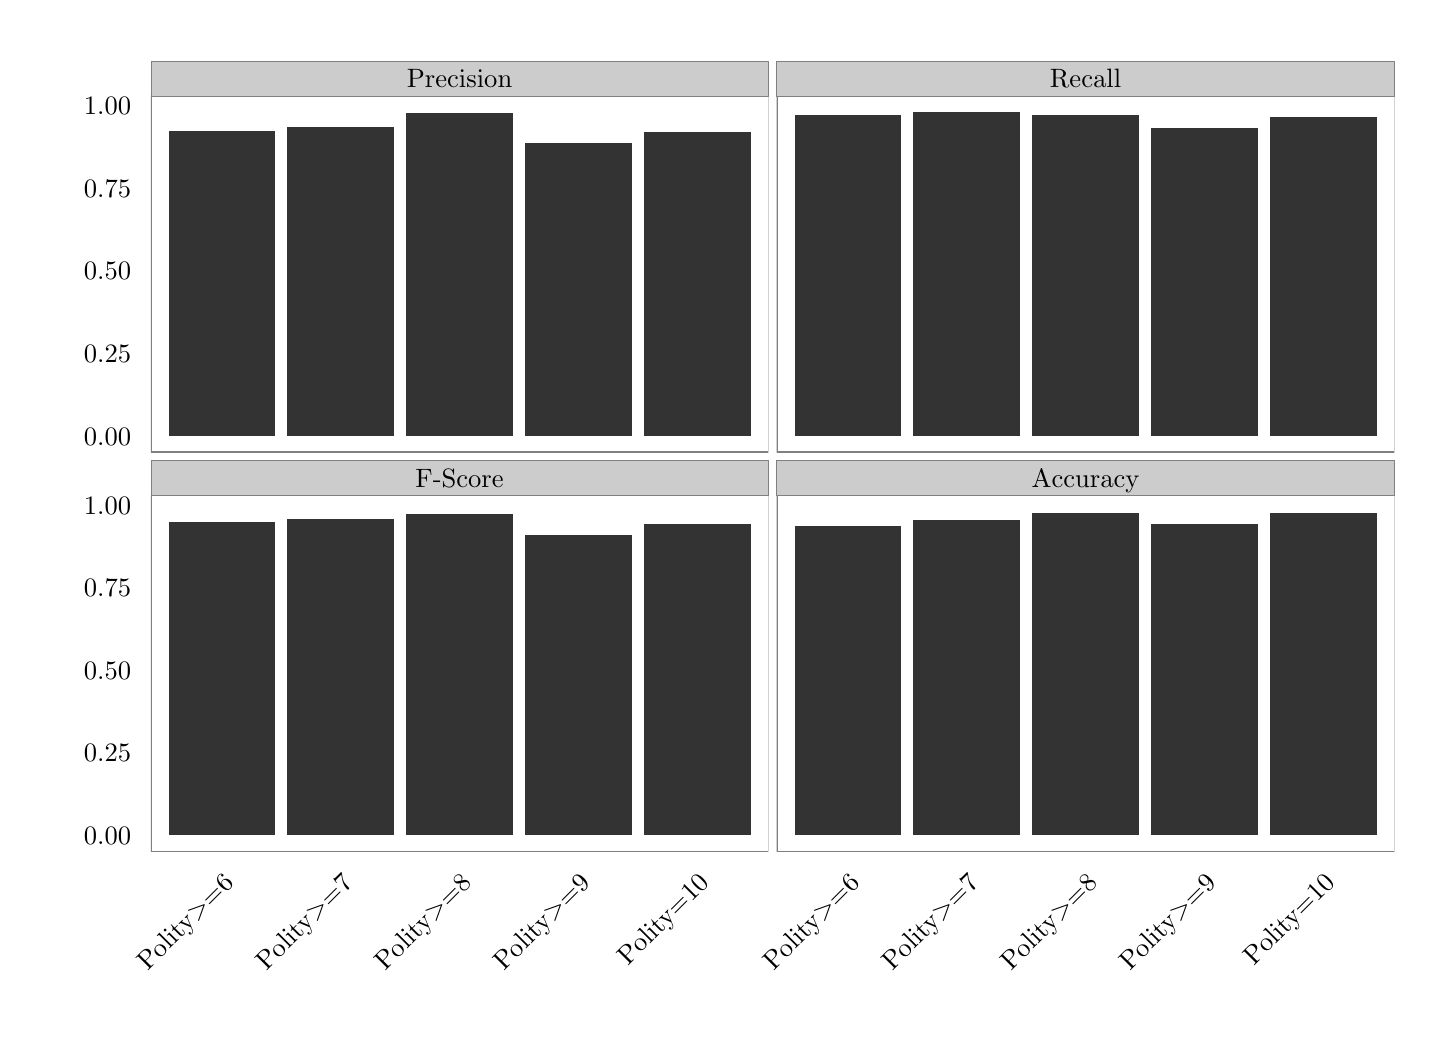
\begin{tikzpicture}[x=1pt,y=1pt]
\definecolor[named]{drawColor}{rgb}{0.00,0.00,0.00}
\definecolor[named]{fillColor}{rgb}{1.00,1.00,1.00}
\fill[color=fillColor,fill opacity=0.00,] (0,0) rectangle (505.89,361.35);
\begin{scope}
\path[clip] (  0.00,  0.00) rectangle (505.89,361.35);
\end{scope}
\begin{scope}
\path[clip] (  0.00,  0.00) rectangle (505.89,361.35);
\end{scope}
\begin{scope}
\path[clip] (  0.00,  0.00) rectangle (505.89,361.35);
\definecolor[named]{drawColor}{rgb}{1.00,1.00,1.00}
\definecolor[named]{fillColor}{rgb}{1.00,1.00,1.00}

\draw[color=drawColor,line width= 0.6pt,line cap=round,line join=round,fill=fillColor,] (  0.00,  0.00) rectangle (505.89,361.35);
\end{scope}
\begin{scope}
\path[clip] (  0.00,  0.00) rectangle (505.89,361.35);
\end{scope}
\begin{scope}
\path[clip] ( 44.49,208.00) rectangle (267.66,336.67);
\definecolor[named]{fillColor}{rgb}{1.00,1.00,1.00}

\draw[fill=fillColor,draw opacity=0.00,] ( 44.49,208.00) rectangle (267.66,336.67);
\definecolor[named]{fillColor}{rgb}{0.20,0.20,0.20}

\draw[fill=fillColor,draw opacity=0.00,] ( 50.92,213.85) rectangle ( 89.55,324.02);

\draw[fill=fillColor,draw opacity=0.00,] ( 93.84,213.85) rectangle (132.47,325.52);

\draw[fill=fillColor,draw opacity=0.00,] (136.76,213.85) rectangle (175.39,330.43);

\draw[fill=fillColor,draw opacity=0.00,] (179.68,213.85) rectangle (218.30,319.67);

\draw[fill=fillColor,draw opacity=0.00,] (222.60,213.85) rectangle (261.22,323.67);
\definecolor[named]{drawColor}{rgb}{0.50,0.50,0.50}

\draw[color=drawColor,line width= 0.6pt,line cap=round,line join=round,fill opacity=0.00,] ( 44.49,208.00) rectangle (267.66,336.67);
\end{scope}
\begin{scope}
\path[clip] (  0.00,  0.00) rectangle (505.89,361.35);
\end{scope}
\begin{scope}
\path[clip] (270.67,208.00) rectangle (493.85,336.67);
\definecolor[named]{fillColor}{rgb}{1.00,1.00,1.00}

\draw[fill=fillColor,draw opacity=0.00,] (270.67,208.00) rectangle (493.85,336.67);
\definecolor[named]{fillColor}{rgb}{0.20,0.20,0.20}

\draw[fill=fillColor,draw opacity=0.00,] (277.11,213.85) rectangle (315.73,329.95);

\draw[fill=fillColor,draw opacity=0.00,] (320.03,213.85) rectangle (358.65,330.82);

\draw[fill=fillColor,draw opacity=0.00,] (362.94,213.85) rectangle (401.57,329.68);

\draw[fill=fillColor,draw opacity=0.00,] (405.86,213.85) rectangle (444.49,324.98);

\draw[fill=fillColor,draw opacity=0.00,] (448.78,213.85) rectangle (487.41,329.01);
\definecolor[named]{drawColor}{rgb}{0.50,0.50,0.50}

\draw[color=drawColor,line width= 0.6pt,line cap=round,line join=round,fill opacity=0.00,] (270.67,208.00) rectangle (493.85,336.67);
\end{scope}
\begin{scope}
\path[clip] (  0.00,  0.00) rectangle (505.89,361.35);
\end{scope}
\begin{scope}
\path[clip] ( 44.49, 63.68) rectangle (267.66,192.35);
\definecolor[named]{fillColor}{rgb}{1.00,1.00,1.00}

\draw[fill=fillColor,draw opacity=0.00,] ( 44.49, 63.68) rectangle (267.66,192.35);
\definecolor[named]{fillColor}{rgb}{0.20,0.20,0.20}

\draw[fill=fillColor,draw opacity=0.00,] ( 50.92, 69.53) rectangle ( 89.55,182.59);

\draw[fill=fillColor,draw opacity=0.00,] ( 93.84, 69.53) rectangle (132.47,183.79);

\draw[fill=fillColor,draw opacity=0.00,] (136.76, 69.53) rectangle (175.39,185.74);

\draw[fill=fillColor,draw opacity=0.00,] (179.68, 69.53) rectangle (218.30,177.94);

\draw[fill=fillColor,draw opacity=0.00,] (222.60, 69.53) rectangle (261.22,181.96);
\definecolor[named]{drawColor}{rgb}{0.50,0.50,0.50}

\draw[color=drawColor,line width= 0.6pt,line cap=round,line join=round,fill opacity=0.00,] ( 44.49, 63.68) rectangle (267.66,192.35);
\end{scope}
\begin{scope}
\path[clip] (  0.00,  0.00) rectangle (505.89,361.35);
\end{scope}
\begin{scope}
\path[clip] (270.67, 63.68) rectangle (493.85,192.35);
\definecolor[named]{fillColor}{rgb}{1.00,1.00,1.00}

\draw[fill=fillColor,draw opacity=0.00,] (270.67, 63.68) rectangle (493.85,192.35);
\definecolor[named]{fillColor}{rgb}{0.20,0.20,0.20}

\draw[fill=fillColor,draw opacity=0.00,] (277.11, 69.53) rectangle (315.73,181.41);

\draw[fill=fillColor,draw opacity=0.00,] (320.03, 69.53) rectangle (358.65,183.60);

\draw[fill=fillColor,draw opacity=0.00,] (362.94, 69.53) rectangle (401.57,186.14);

\draw[fill=fillColor,draw opacity=0.00,] (405.86, 69.53) rectangle (444.49,181.92);

\draw[fill=fillColor,draw opacity=0.00,] (448.78, 69.53) rectangle (487.41,185.97);
\definecolor[named]{drawColor}{rgb}{0.50,0.50,0.50}

\draw[color=drawColor,line width= 0.6pt,line cap=round,line join=round,fill opacity=0.00,] (270.67, 63.68) rectangle (493.85,192.35);
\end{scope}
\begin{scope}
\path[clip] (  0.00,  0.00) rectangle (505.89,361.35);
\end{scope}
\begin{scope}
\path[clip] (  0.00,  0.00) rectangle (505.89,361.35);
\definecolor[named]{drawColor}{rgb}{0.50,0.50,0.50}
\definecolor[named]{fillColor}{rgb}{0.80,0.80,0.80}

\draw[color=drawColor,line width= 0.2pt,line cap=round,line join=round,fill=fillColor,] ( 44.49,336.67) rectangle (267.66,349.31);
\definecolor[named]{drawColor}{rgb}{0.00,0.00,0.00}

\node[color=drawColor,anchor=base,inner sep=0pt, outer sep=0pt, scale=  0.96] at (156.07,339.68) {Precision};
\end{scope}
\begin{scope}
\path[clip] (  0.00,  0.00) rectangle (505.89,361.35);
\end{scope}
\begin{scope}
\path[clip] (  0.00,  0.00) rectangle (505.89,361.35);
\definecolor[named]{drawColor}{rgb}{0.50,0.50,0.50}
\definecolor[named]{fillColor}{rgb}{0.80,0.80,0.80}

\draw[color=drawColor,line width= 0.2pt,line cap=round,line join=round,fill=fillColor,] (270.67,336.67) rectangle (493.85,349.31);
\definecolor[named]{drawColor}{rgb}{0.00,0.00,0.00}

\node[color=drawColor,anchor=base,inner sep=0pt, outer sep=0pt, scale=  0.96] at (382.26,339.68) {Recall};
\end{scope}
\begin{scope}
\path[clip] (  0.00,  0.00) rectangle (505.89,361.35);
\end{scope}
\begin{scope}
\path[clip] (  0.00,  0.00) rectangle (505.89,361.35);
\definecolor[named]{drawColor}{rgb}{0.50,0.50,0.50}
\definecolor[named]{fillColor}{rgb}{0.80,0.80,0.80}

\draw[color=drawColor,line width= 0.2pt,line cap=round,line join=round,fill=fillColor,] ( 44.49,192.35) rectangle (267.66,204.99);
\definecolor[named]{drawColor}{rgb}{0.00,0.00,0.00}

\node[color=drawColor,anchor=base,inner sep=0pt, outer sep=0pt, scale=  0.96] at (156.07,195.36) {F-Score};
\end{scope}
\begin{scope}
\path[clip] (  0.00,  0.00) rectangle (505.89,361.35);
\end{scope}
\begin{scope}
\path[clip] (  0.00,  0.00) rectangle (505.89,361.35);
\definecolor[named]{drawColor}{rgb}{0.50,0.50,0.50}
\definecolor[named]{fillColor}{rgb}{0.80,0.80,0.80}

\draw[color=drawColor,line width= 0.2pt,line cap=round,line join=round,fill=fillColor,] (270.67,192.35) rectangle (493.85,204.99);
\definecolor[named]{drawColor}{rgb}{0.00,0.00,0.00}

\node[color=drawColor,anchor=base,inner sep=0pt, outer sep=0pt, scale=  0.96] at (382.26,195.36) {Accuracy};
\end{scope}
\begin{scope}
\path[clip] (  0.00,  0.00) rectangle (505.89,361.35);
\end{scope}
\begin{scope}
\path[clip] (  0.00,  0.00) rectangle (505.89,361.35);
\end{scope}
\begin{scope}
\path[clip] (  0.00,  0.00) rectangle (505.89,361.35);
\definecolor[named]{drawColor}{rgb}{0.00,0.00,0.00}

\node[color=drawColor,anchor=base east,inner sep=0pt, outer sep=0pt, scale=  0.96] at ( 37.37,210.54) {0.00};

\node[color=drawColor,anchor=base east,inner sep=0pt, outer sep=0pt, scale=  0.96] at ( 37.37,240.37) {0.25};

\node[color=drawColor,anchor=base east,inner sep=0pt, outer sep=0pt, scale=  0.96] at ( 37.37,270.19) {0.50};

\node[color=drawColor,anchor=base east,inner sep=0pt, outer sep=0pt, scale=  0.96] at ( 37.37,300.02) {0.75};

\node[color=drawColor,anchor=base east,inner sep=0pt, outer sep=0pt, scale=  0.96] at ( 37.37,329.85) {1.00};
\end{scope}
\begin{scope}
\path[clip] (  0.00,  0.00) rectangle (505.89,361.35);
\end{scope}
\begin{scope}
\path[clip] (  0.00,  0.00) rectangle (505.89,361.35);
\end{scope}
\begin{scope}
\path[clip] (  0.00,  0.00) rectangle (505.89,361.35);
\end{scope}
\begin{scope}
\path[clip] (  0.00,  0.00) rectangle (505.89,361.35);
\end{scope}
\begin{scope}
\path[clip] (  0.00,  0.00) rectangle (505.89,361.35);
\end{scope}
\begin{scope}
\path[clip] (  0.00,  0.00) rectangle (505.89,361.35);
\end{scope}
\begin{scope}
\path[clip] (  0.00,  0.00) rectangle (505.89,361.35);
\end{scope}
\begin{scope}
\path[clip] (  0.00,  0.00) rectangle (505.89,361.35);
\end{scope}
\begin{scope}
\path[clip] (  0.00,  0.00) rectangle (505.89,361.35);
\end{scope}
\begin{scope}
\path[clip] (  0.00,  0.00) rectangle (505.89,361.35);
\definecolor[named]{drawColor}{rgb}{0.00,0.00,0.00}

\node[color=drawColor,anchor=base east,inner sep=0pt, outer sep=0pt, scale=  0.96] at ( 37.37, 66.22) {0.00};

\node[color=drawColor,anchor=base east,inner sep=0pt, outer sep=0pt, scale=  0.96] at ( 37.37, 96.05) {0.25};

\node[color=drawColor,anchor=base east,inner sep=0pt, outer sep=0pt, scale=  0.96] at ( 37.37,125.87) {0.50};

\node[color=drawColor,anchor=base east,inner sep=0pt, outer sep=0pt, scale=  0.96] at ( 37.37,155.70) {0.75};

\node[color=drawColor,anchor=base east,inner sep=0pt, outer sep=0pt, scale=  0.96] at ( 37.37,185.53) {1.00};
\end{scope}
\begin{scope}
\path[clip] (  0.00,  0.00) rectangle (505.89,361.35);
\end{scope}
\begin{scope}
\path[clip] (  0.00,  0.00) rectangle (505.89,361.35);
\end{scope}
\begin{scope}
\path[clip] (  0.00,  0.00) rectangle (505.89,361.35);
\end{scope}
\begin{scope}
\path[clip] (  0.00,  0.00) rectangle (505.89,361.35);
\end{scope}
\begin{scope}
\path[clip] (  0.00,  0.00) rectangle (505.89,361.35);
\end{scope}
\begin{scope}
\path[clip] (  0.00,  0.00) rectangle (505.89,361.35);
\end{scope}
\begin{scope}
\path[clip] (  0.00,  0.00) rectangle (505.89,361.35);
\end{scope}
\begin{scope}
\path[clip] (  0.00,  0.00) rectangle (505.89,361.35);
\end{scope}
\begin{scope}
\path[clip] (  0.00,  0.00) rectangle (505.89,361.35);
\end{scope}
\begin{scope}
\path[clip] (  0.00,  0.00) rectangle (505.89,361.35);
\end{scope}
\begin{scope}
\path[clip] (  0.00,  0.00) rectangle (505.89,361.35);
\end{scope}
\begin{scope}
\path[clip] (  0.00,  0.00) rectangle (505.89,361.35);
\end{scope}
\begin{scope}
\path[clip] (  0.00,  0.00) rectangle (505.89,361.35);
\end{scope}
\begin{scope}
\path[clip] (  0.00,  0.00) rectangle (505.89,361.35);
\end{scope}
\begin{scope}
\path[clip] (  0.00,  0.00) rectangle (505.89,361.35);
\end{scope}
\begin{scope}
\path[clip] (  0.00,  0.00) rectangle (505.89,361.35);
\definecolor[named]{drawColor}{rgb}{0.00,0.00,0.00}

\node[rotate= 45.00,color=drawColor,anchor=base east,inner sep=0pt, outer sep=0pt, scale=  0.96] at ( 74.91, 51.89) {Polity$>=$6};

\node[rotate= 45.00,color=drawColor,anchor=base east,inner sep=0pt, outer sep=0pt, scale=  0.96] at (117.83, 51.89) {Polity$>=$7};

\node[rotate= 45.00,color=drawColor,anchor=base east,inner sep=0pt, outer sep=0pt, scale=  0.96] at (160.75, 51.89) {Polity$>=$8};

\node[rotate= 45.00,color=drawColor,anchor=base east,inner sep=0pt, outer sep=0pt, scale=  0.96] at (203.67, 51.89) {Polity$>=$9};

\node[rotate= 45.00,color=drawColor,anchor=base east,inner sep=0pt, outer sep=0pt, scale=  0.96] at (246.58, 51.89) {Polity$=$10};
\end{scope}
\begin{scope}
\path[clip] (  0.00,  0.00) rectangle (505.89,361.35);
\end{scope}
\begin{scope}
\path[clip] (  0.00,  0.00) rectangle (505.89,361.35);
\end{scope}
\begin{scope}
\path[clip] (  0.00,  0.00) rectangle (505.89,361.35);
\end{scope}
\begin{scope}
\path[clip] (  0.00,  0.00) rectangle (505.89,361.35);
\end{scope}
\begin{scope}
\path[clip] (  0.00,  0.00) rectangle (505.89,361.35);
\end{scope}
\begin{scope}
\path[clip] (  0.00,  0.00) rectangle (505.89,361.35);
\end{scope}
\begin{scope}
\path[clip] (  0.00,  0.00) rectangle (505.89,361.35);
\end{scope}
\begin{scope}
\path[clip] (  0.00,  0.00) rectangle (505.89,361.35);
\definecolor[named]{drawColor}{rgb}{0.00,0.00,0.00}

\node[rotate= 45.00,color=drawColor,anchor=base east,inner sep=0pt, outer sep=0pt, scale=  0.96] at (301.10, 51.89) {Polity$>=$6};

\node[rotate= 45.00,color=drawColor,anchor=base east,inner sep=0pt, outer sep=0pt, scale=  0.96] at (344.02, 51.89) {Polity$>=$7};

\node[rotate= 45.00,color=drawColor,anchor=base east,inner sep=0pt, outer sep=0pt, scale=  0.96] at (386.93, 51.89) {Polity$>=$8};

\node[rotate= 45.00,color=drawColor,anchor=base east,inner sep=0pt, outer sep=0pt, scale=  0.96] at (429.85, 51.89) {Polity$>=$9};

\node[rotate= 45.00,color=drawColor,anchor=base east,inner sep=0pt, outer sep=0pt, scale=  0.96] at (472.77, 51.89) {Polity$=$10};
\end{scope}
\begin{scope}
\path[clip] (  0.00,  0.00) rectangle (505.89,361.35);
\end{scope}
\begin{scope}
\path[clip] (  0.00,  0.00) rectangle (505.89,361.35);
\end{scope}
\begin{scope}
\path[clip] (  0.00,  0.00) rectangle (505.89,361.35);
\end{scope}
\begin{scope}
\path[clip] (  0.00,  0.00) rectangle (505.89,361.35);
\end{scope}
\begin{scope}
\path[clip] (  0.00,  0.00) rectangle (505.89,361.35);
\end{scope}
\begin{scope}
\path[clip] (  0.00,  0.00) rectangle (505.89,361.35);
\end{scope}
\begin{scope}
\path[clip] (  0.00,  0.00) rectangle (505.89,361.35);
\end{scope}
\begin{scope}
\path[clip] (  0.00,  0.00) rectangle (505.89,361.35);
\end{scope}
\begin{scope}
\path[clip] (  0.00,  0.00) rectangle (505.89,361.35);
\end{scope}
\begin{scope}
\path[clip] (  0.00,  0.00) rectangle (505.89,361.35);
\end{scope}
\begin{scope}
\path[clip] (  0.00,  0.00) rectangle (505.89,361.35);
\end{scope}
\end{tikzpicture}
}	
\end{figure}

\end{frame}
%%%%%%%%%%%%%%%%%%%%%%%%%%%%%%%%%%%%%%%%%

%%%%%%%%%%%%%%%%%%%%%%%%%%%%%%%%%%%%%%%%%
\begin{frame}
\frametitle{Performance by Class for Democracy}

\text{\textbf{Naive Bayes}}
\begin{table}[ht]
\centering
\begin{tabular}{lcccc}
\hline\hline
~& Precision & Recall & F-score & Support \\
Not Democracy & 0.96 & 0.90 & 0.93 & 563 \\
Democracy & 0.68 & 0.85 & 0.76 & 144
\end{tabular}
\end{table}

\text{\textbf{SVM}}
\begin{table}[ht]
\centering
\begin{tabular}{lcccc}
\hline\hline
~& Precision & Recall & F-score & Support \\
Not Democracy & 0.99 & 0.98 & 0.98 & 563 \\
Democracy & 0.93 & 0.96 & 0.94 & 144
\end{tabular}
\end{table}

\end{frame}
%%%%%%%%%%%%%%%%%%%%%%%%%%%%%%%%%%%%%%%%%

%%%%%%%%%%%%%%%%%%%%%%%%%%%%%%%%%%%%%%%%%
\begin{frame}
\frametitle{Performance by Class for Military}

\text{\textbf{Naive Bayes}}
\begin{table}[ht]
\centering
\begin{tabular}{lcccc}
\hline\hline
~& Precision & Recall & F-score & Support \\
Not Military & 0.99 & 0.99 & 0.99 & 574 \\
Military & 0.57 & 0.44 & 0.50 & 9
\end{tabular}
\end{table}

\text{\textbf{SVM}}
\begin{table}[ht]
\centering
\begin{tabular}{lcccc}
\hline\hline
~& Precision & Recall & F-score & Support \\
Not Military & 0.99 & 1.00 & 1.00 & 574 \\
Military & 1.00 & 0.67 & 0.80 & 9
\end{tabular}
\end{table}

\end{frame}
%%%%%%%%%%%%%%%%%%%%%%%%%%%%%%%%%%%%%%%%%

%%%%%%%%%%%%%%%%%%%%%%%%%%%%%%%%%%%%%%%%%
\begin{frame}
\frametitle{Performance by Class for Monarchy}

\text{\textbf{Naive Bayes}}
\begin{table}[ht]
\centering
\begin{tabular}{lcccc}
\hline\hline
~& Precision & Recall & F-score & Support \\
Not Monarchy & 0.97 & 1.00 & 0.99 & 557 \\
Monarchy & 1.00 & 0.38 & 0.56 & 26
\end{tabular}
\end{table}

\text{\textbf{SVM}}
\begin{table}[ht]
\centering
\begin{tabular}{lcccc}
\hline\hline
~& Precision & Recall & F-score & Support \\
Not Monarchy & 1.00 & 1.00 & 1.00 & 557 \\
Monarchy & 0.93 & 1.00 & 0.96 & 26
\end{tabular}
\end{table}

\end{frame}
%%%%%%%%%%%%%%%%%%%%%%%%%%%%%%%%%%%%%%%%%

%%%%%%%%%%%%%%%%%%%%%%%%%%%%%%%%%%%%%%%%%
\begin{frame}
\frametitle{Performance by Class for One-Party}

\text{\textbf{Naive Bayes}}
\begin{table}[ht]
\centering
\begin{tabular}{lcccc}
\hline\hline
~& Precision & Recall & F-score & Support \\
Not One-Party & 0.98 & 0.99 & 0.99 & 555 \\
One-Party & 0.83 & 0.54 & 0.65 & 28
\end{tabular}
\end{table}

\text{\textbf{SVM}}
\begin{table}[ht]
\centering
\begin{tabular}{lcccc}
\hline\hline
~& Precision & Recall & F-score & Support \\
Not One-Party & 1.00 & 1.00 & 1.00 & 555 \\
One-Party & 1.00 & 0.93 & 0.96 & 28
\end{tabular}
\end{table}

\end{frame}
%%%%%%%%%%%%%%%%%%%%%%%%%%%%%%%%%%%%%%%%%

%%%%%%%%%%%%%%%%%%%%%%%%%%%%%%%%%%%%%%%%%
\begin{frame}
\frametitle{Next Steps}

\begin{itemize}
	\item Incorporate additional textual data from Human Rights Watch
	\item Compare performance of SVM with supervised LDAs
\end{itemize}

\end{frame}
%%%%%%%%%%%%%%%%%%%%%%%%%%%%%%%%%%%%%%%%%

% End of slides
\end{document} 